\subsection{Sensing}
As the controller required the simultaneous measurement of both the input and output voltages it was important to condition the signals to appropriate levels such that they could be sampled by correctly by the ADC.
\tikzstyle{block} = [rectangle, draw, fill=\myblue, 
    text width=6em, text badly centered, rounded corners, minimum height=4em]
\begin{figure}[H]
\centering
\fbox{
\begin{tikzpicture}[node distance = 1cm]
\node [block, fill=\myblue, text width=4em] (scaling) {scaling};
\node [block, right = of scaling, fill=\myblue, text width=5em] (buffering) {buffering};
\node [block, right = of buffering, fill=\myblue, text width=5em] (gainstage) {gain stage};
\node [block, right = of gainstage, fill=\myblue, text width=6em] (antialiasing) {anti-aliasing};
\node [block, right = of antialiasing, fill=\myblue, text width=5em] (clamping) {clamping};
%
\path [line, ultra thick] (scaling)	-- (buffering);
\path [line, ultra thick] (buffering) -- (gainstage);
\path [line, ultra thick] (gainstage) -- (antialiasing);
\path [line, ultra thick] (antialiasing) -- (clamping);
\end{tikzpicture}
}
\caption{Voltage sensing system architecture.}
\label{fig:sensing_system}
\end{figure}
The expected voltages and frequency content of the input and output are different and hence need to be designed separately. Both signals must past through five stages (see figure \ref{fig:sensing_system}) before they are appropriate to be sampled by the ADC; each stage will be outlined in detail below. First, we must outline the characteristics of the two signals that we wish to measure.

\paragraph{Input voltage}
The input of the \'Cuk Converter is directly connected to the top of the ultra-capacitor stack. Hence, we can expect a slowly varying signal that is between \SI{0}{V} and \SI{5}{V}. The frequency content of this voltage will be low frequency and hence a low order passive anti-aliasing filter will be appropriate. It should also be noted that this signal if positive with respect to ground and hence will not require inversion.
\begin{figure}[H]
    \centering
    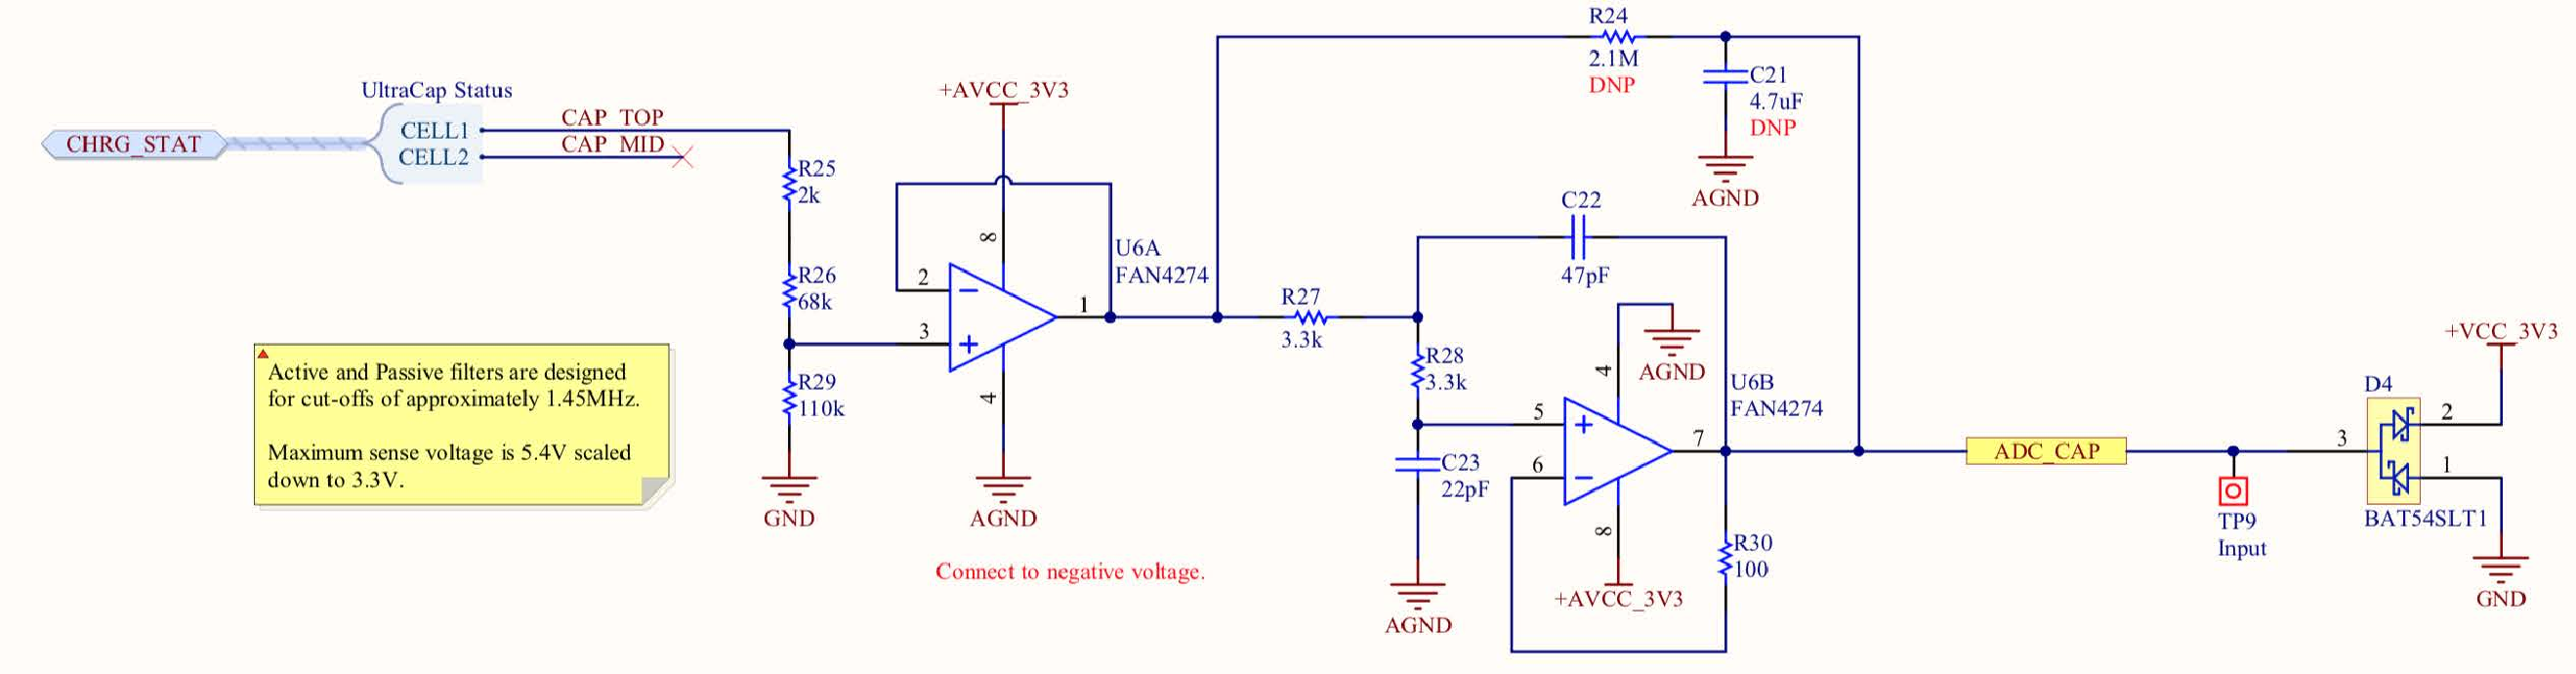
\includegraphics[width = 14cm]{figures/hardware/input_sense.pdf}
    \caption{Converter input voltage schematic excerpt.}
    \label{fig:input_sense}
\end{figure}

\paragraph{Output voltage}
The output of the \'Cuk Conveter is significantly more complicated than the input. It contains high frequency switching content from the MOSFET switching at a nominal \SI{100}{kHz} and will also contain fast transient due to the control action. It is vital that this information is preserved for optimal performance of the controller. To preserve as much of the high frequency we must use a higher order active filter with a smaller transition region around the Nyquist frequency.

As the \'Cuk Converter topology produces an inverted output voltage with respect to ground, care must be taken to invert this signal such that it can be sampled correctly by the ADC. The MCU contains a rail-to-rail analog to digital converter (ADC) and hence can sample voltages between 0 and \SI{3}{V} (positive). Hence a gain stage must include a negative gain such that the voltage is positive. As theoretically the output of the converter can be anything that we choose it to be, it was decided to specify and support output voltages between $-\SI{15}{V}$ and \SI{0}{V}.
\begin{figure}[H]
    \centering
    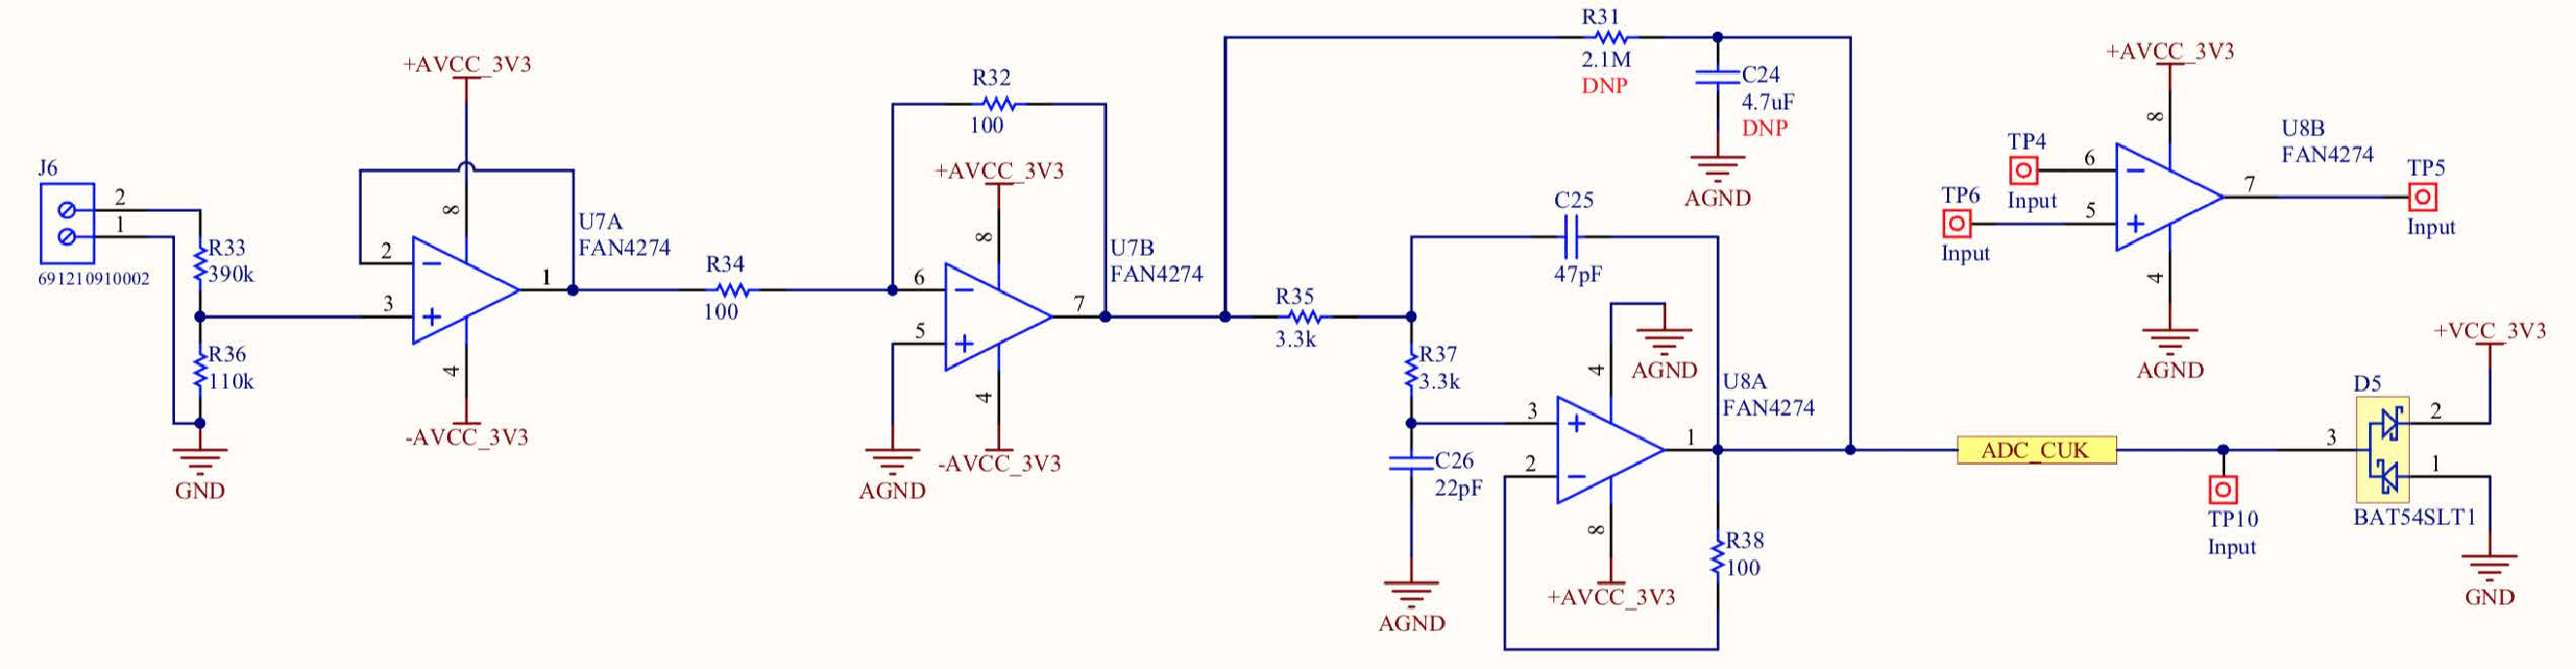
\includegraphics[width = 14cm]{figures/hardware/output_sense.pdf}
    \caption{Converter output voltage schematic excerpt.}
    \label{fig:output_sense}
\end{figure}

\subsubsection{Scaling}
As the chosen microcontroller can only sample voltages from \SI{0}{V} to \SI{3.3}{V}, we must scale the voltage of both the input and output such that the voltage is between these stages. To ensure maximum resolution of the sampled voltage and avoid quantisation from affecting the measurements it was important to ensure that the voltages could swing between the \SI{0}{V} and \SI{3.3}{V} range without experiencing clipping. To achieve this a resistive divider was employed to scale the voltage down by a set factor.
\\ \\
In order to reduce power loses the quiescent current must be traded off with the loading of the operation amplifier. Using too low of a resistance for the divider would result in high quiescent currents and hence large power loses, too high of a resistance would being to be loaded by the operational amplifier. As the input impedance of an operational amplifier is unknown and varies significantly between devices, by design, we are unable to compensate for the loading and thereby the accuracy of the measurements will be affected. We found that choosing resistors in the \SI{100}{k\ohm} range performed well. It was also essential that low tolerance ($\pm0.1 \%$) resistances were chosen such that accuracy could be maintained.
\\ \\
Once the voltages were scaled, they would be re-scaled inside the microcontroller by multiplying by a constant factor that divided on the resistors used in the voltage divider. If these resistances themselves where not known to a high degree of accuracy this scaling factor would be significantly out of specification.

\subsubsection{Buffer}
So that the voltage divider was not loaded by the filter stage and affecting the accuracy of the results. The resistances of the filters were chosen to be of a similar order of magnitude to the resistive divider to avoid current saturation of the operational amplifiers and to minimise power losses, hence loading was a real concern.
\\ \\
By including an operational amplifier configured as a buffer the high impedance input and low impendence output would avoid loading of either stage.


\subsubsection{Gain Stage}
As the output voltage of the \'Cuk converter is negative an operational amplifier configured as a unity gain inverting amplifier was required.

%Initially the resistances chosen for the feedback weas too small resulting in current saturation of the op amp. Too much current was being drawn from the buffer stage causing the voltage to saturate around 2.2V.

\subsubsection{Anti-aliasing filter}
The input and the output of the DC-DC converter must pass through an anti-aliasing filter such that any high frequency content is removed before the signal is sampled by the ADC. Failure to remove this high-frequency noise results in folding and will corrupt the low frequency content. Since the output has a lot of high frequency content, ripple and transients that should be measured it is important that the AA filter has a fast roll off to ensure as much of this signal is preserved as possible. For the input, this isn’t as important. It is slowly varying, hence a first order passive filter was employed instead.
\\ \\
``A practical anti-aliasing filter should have a magnitude response approximately unity in the passband, a stopband response exceeding a minimum attenuation level and an acceptable transistion band separating the passband and stopband.'' \cite{dsp} A butterworth low pass filter meets these requires and was designed using the Sallen Key topology for a cut-off at Nyquist rate \SI{5}{kHz}. The topology and component values are shown in figure \ref{fig:output_sense}.

\subsubsection{Clamping}
To ensure the pins of the microcontroller and not destroyed by exceeding their maximum voltage rating, diodes were employed to clamp the voltages to within a fixed range. If a voltage exceed \SI{3.3}{V} plus the forward voltage of the diode, the diode would appear as a short circuit to the signal and hence any potentially damaging voltages would appear across the diodes rather than the microcontroller pins.

\subsubsection{Operation amplifier}
The main deciding factor for operational amplifier with a large gain bandwidth product. This was due to a the sampling frequency being unspecified while the control algorithm was being designed and also to due to a lack of understanding in regards to how high frequency content affect the performance of the controller. Hence an operational amplifier was chosen such that it exceeds the half the maximum sampling rate of the ADC.
\\ \\
The FAN4274 from ON Semiconductor provided the performance we required while also offering dual operational amplifiers in the single package, reducing board space \cite{fan4274}.
\\ \\
Despite having a \SI{5}{V} rail, the operational amplifiers were supplied by $\pm\SI{3.3}{V}$ as the $\pm{5}{V}$ would not provide any extra resolution to the ADC and simply result in additional power losses.